
\begin{frame}{Theoretical Background}{Basic aerodynamics and airfoil theory}
	1D momentum theory:
	\begin{itemize}
		\item Air slows down due to delivery of energy from air to rotor blades
		\item Air expands due to conservation of mass
	\end{itemize}
	\begin{figure}[ht]
		\centering
		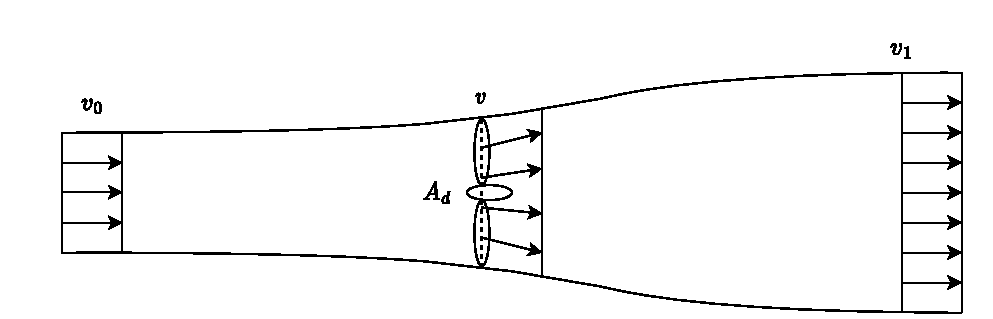
\includegraphics[width=1\linewidth]{../Graphics/FlowThroughRotor.pdf}
		\label{fig:betz}
	\end{figure}
\end{frame}

%%%%%%%%%%%%%%%%%%

\begin{frame}{Theoretical Background}{Basic aerodynamics and airfoil theory}
	Power of wind moving through rotor:
	\begin{equation} \label{eq:power}
		P_{air} = \dfrac{1}{2} \dot{m} \, v_0^2 = \dfrac{1}{2}\rho \, A_d v_0^3
	\end{equation}
	Extractable power defined by \textit{power coefficient} $ C_p $:
	\begin{equation}\label{eq:power_w_Cp}
		P_{T} = \dfrac{1}{2} \rho \, A_d v_0^3 C_p(\theta, \lambda)
	\end{equation}
	where $ \lambda $ is the tip-speed ratio (TSR):
	\begin{equation}\label{key}
		\lambda = \dfrac{R \Omega}{v_0}
	\end{equation}
	The theoretically highest achievable $ C_p $ is the \textit{betz limit}:
	\begin{equation}\label{eq:betzlimit}
		C_{pbetz} = 0.5962
	\end{equation}
	The optimal $ C_p $ for a given turbine is achieved at specific TSR and $ \theta $:
	\begin{equation}\label{eq:cp_optimal}
		C_p^\star = C_p(\theta^\star, \lambda^\star)
	\end{equation}
\end{frame}

%%%%%%%%%%%%%%%%%%

\begin{frame}{Theoretical Background}{Blade element theory}
	\begin{itemize}
		\item Forces are calculated on blade sections (a)
		\item Thrust and torque calculated from velocity triangle (b)
	\end{itemize}

	\begin{equation}
		F_L = \dfrac{1}{2}\,  \rho \, V^2 c \, C_L \;\; , \;\; F_D = \dfrac{1}{2} \, \rho \, V^2 c \, C_D
	\end{equation}
	\begin{equation}
		F_T = F_L \, cos(\phi) + F_D \, sin(\phi) \;\; , \;\;F_Q = F_L \, sin(\phi) - F_D \, cos(\phi)
	\end{equation}
	\begin{figure}[ht]
		\centering
		\subfloat[Blade cross section]{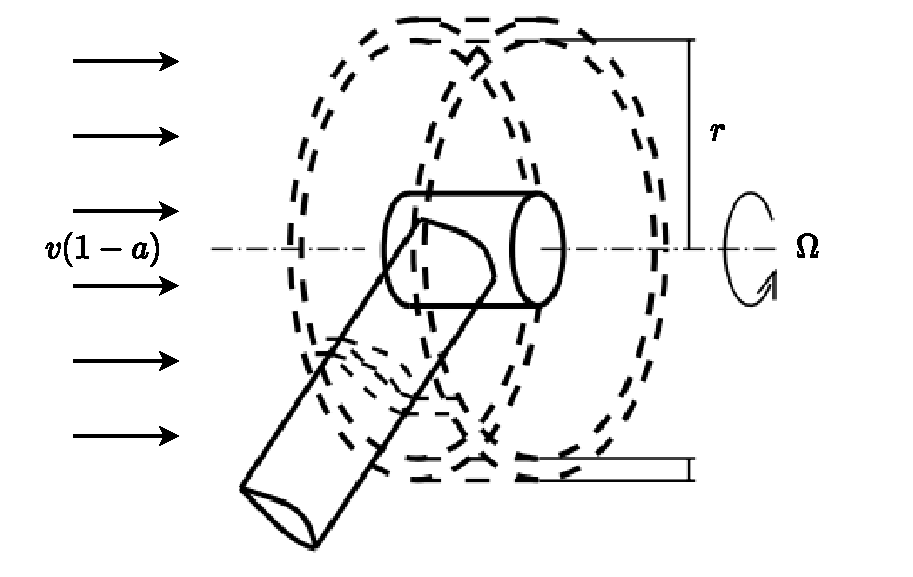
\includegraphics[width=.44\textwidth]{../Graphics/RotorBladeElement.pdf}%
			\label{fig:blade_vel_triangles}}
		\hfil
		\subfloat[Velocity triangle]{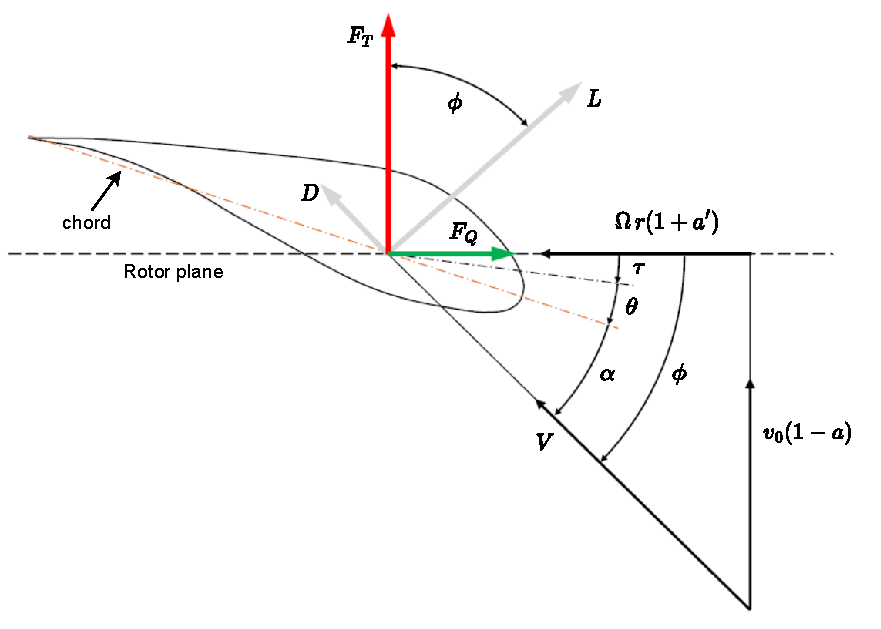
\includegraphics[width=.55\textwidth]{../Graphics/BladeVelocityTriangle.pdf}%
			\label{fig:blade_vel_triangle}}
		\label{fig:blade_triangles}
	\end{figure}
\end{frame}

%%%%%%%%%%%%%%%%%%

\begin{frame}{Theoretical Background}{Wind turbine control}
	Basic turbine controller:
	\begin{figure}[ht]
		\centering
		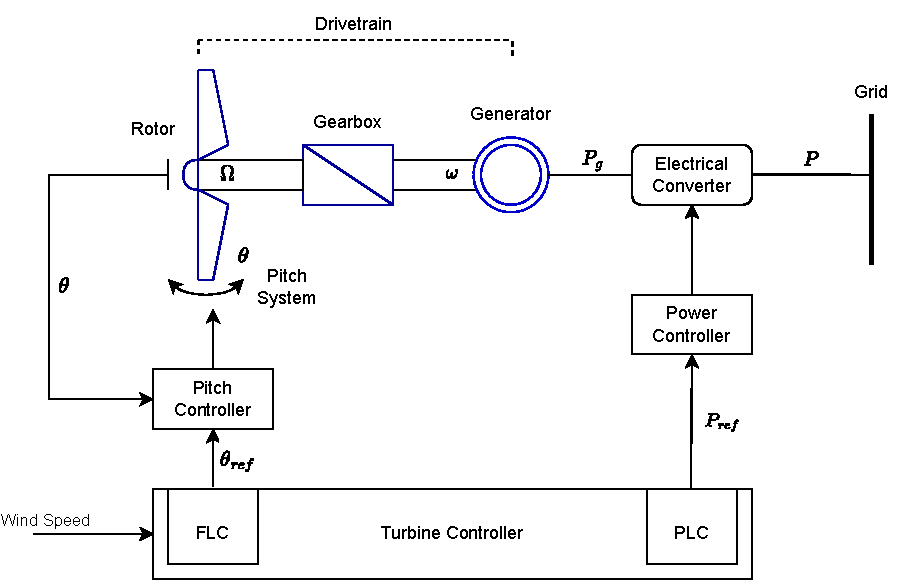
\includegraphics[width=.8\linewidth]{../Graphics/PLC_PI.pdf}
		\label{fig:controller_overview}
	\end{figure}
\end{frame}

%%%%%%%%%%%%%%%%%%

\begin{frame}{Theoretical Background}{Wind turbine control}
	
	\begin{itemize}
		\item Partial load control (PCL): Cut-in to nominal wind speed
		\begin{itemize}
			\item Divided into three subregions
			\item Speed regulated with generator power $ P_g $
		\end{itemize}
		\item Full load control (FLC): Nominal to cut-out wind speed
		\begin{itemize}
			\item Speed regulated with pitch angle $ \theta $
			\item Project focus is on FLC
		\end{itemize}
	\end{itemize}
	\begin{figure}[ht]
		\centering
		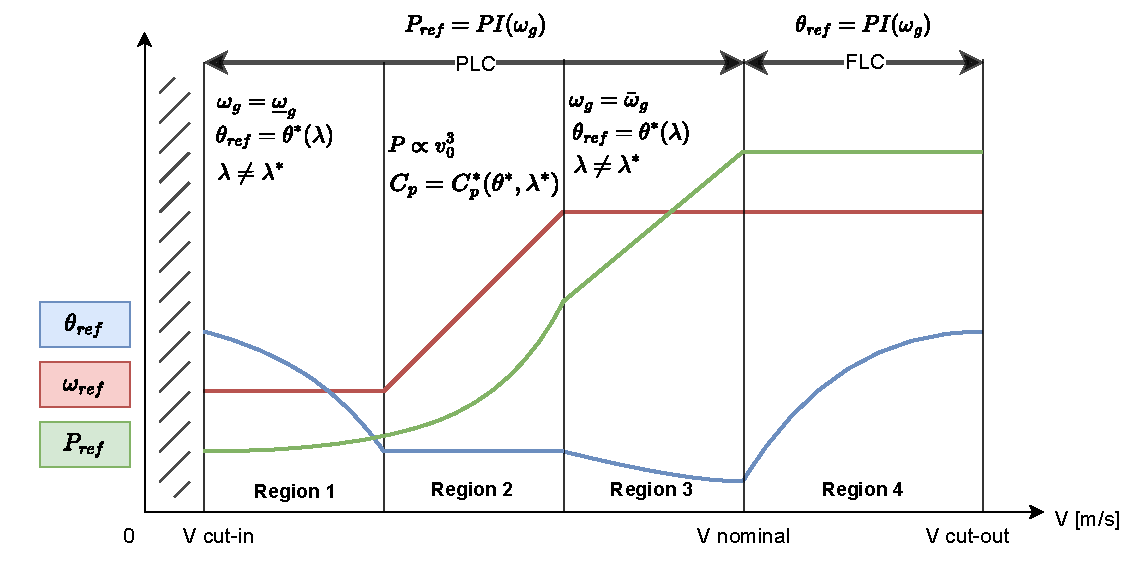
\includegraphics[width=1\linewidth]{../Graphics/OperatingRegions.pdf}
		\label{fig:operating_regions}
	\end{figure}
	Constraints: minimum and maximum speeds: $ \underline \omega $ and $ \bar \omega $
\end{frame}

%%%%%%%%%%%%%%%%%%

\begin{frame}{Theoretical Background}{Partial load control}
	\begin{equation}\label{eq:rotor_speed_deriv}
		\dot{\Omega} = \dfrac{1}{J} \left( T_r(\theta, v_0) - T_g(P_g, \omega) \right) \;\; , \;\; T_g = \dfrac{P_g}{\omega} 
	\end{equation}
	\begin{equation}\label{eq:pi_plc_ctrl}
		P_{ref} = K_{gs}(\omega) \left(K_{plc,P} \, \omega_e + K_{plc,I} \int \omega_e\right) \;\; , \;\; K_{gs}(\omega) = \omega
	\end{equation}
	Main goal: Maximize $ C_p(\theta, \lambda(\Omega, v_0)) $ by setting $ \omega_{ref} = v_0 \lambda^* R^{-1} $
	
	\smallskip
	$ C_p $ plotted against $ \theta $ and $ \lambda $:
	\begin{figure}[ht]
		\centering
		
		\subfloat
		{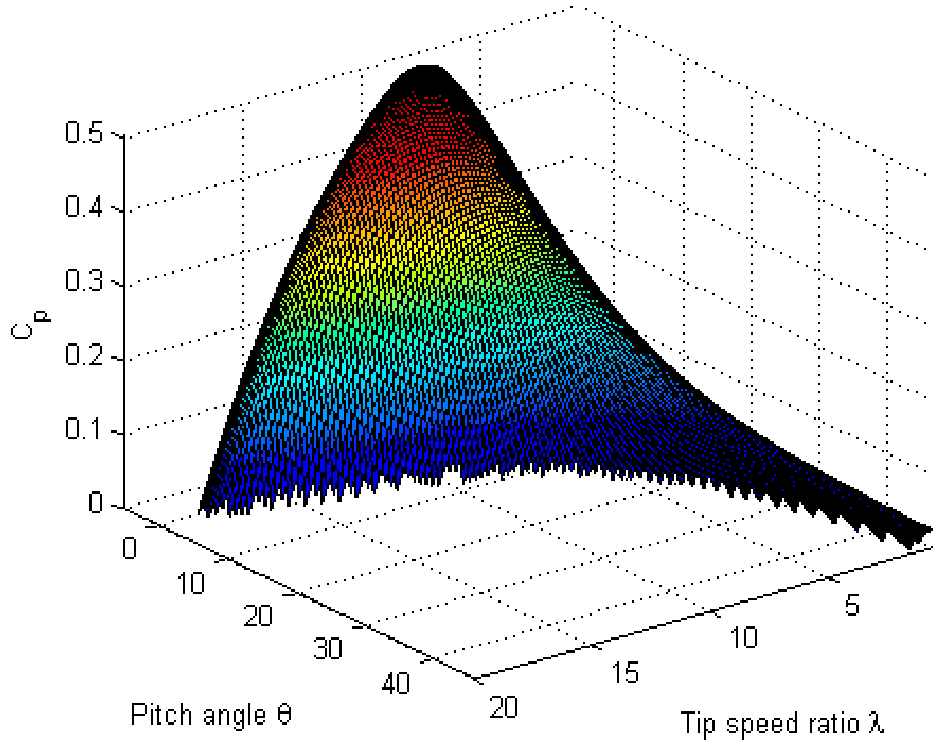
\includegraphics[width=.53\textwidth]{../Graphics/Cp3dPlotV2.png}%
			\label{fig:cp_plot3d}}
		\hfil
		\subfloat
		{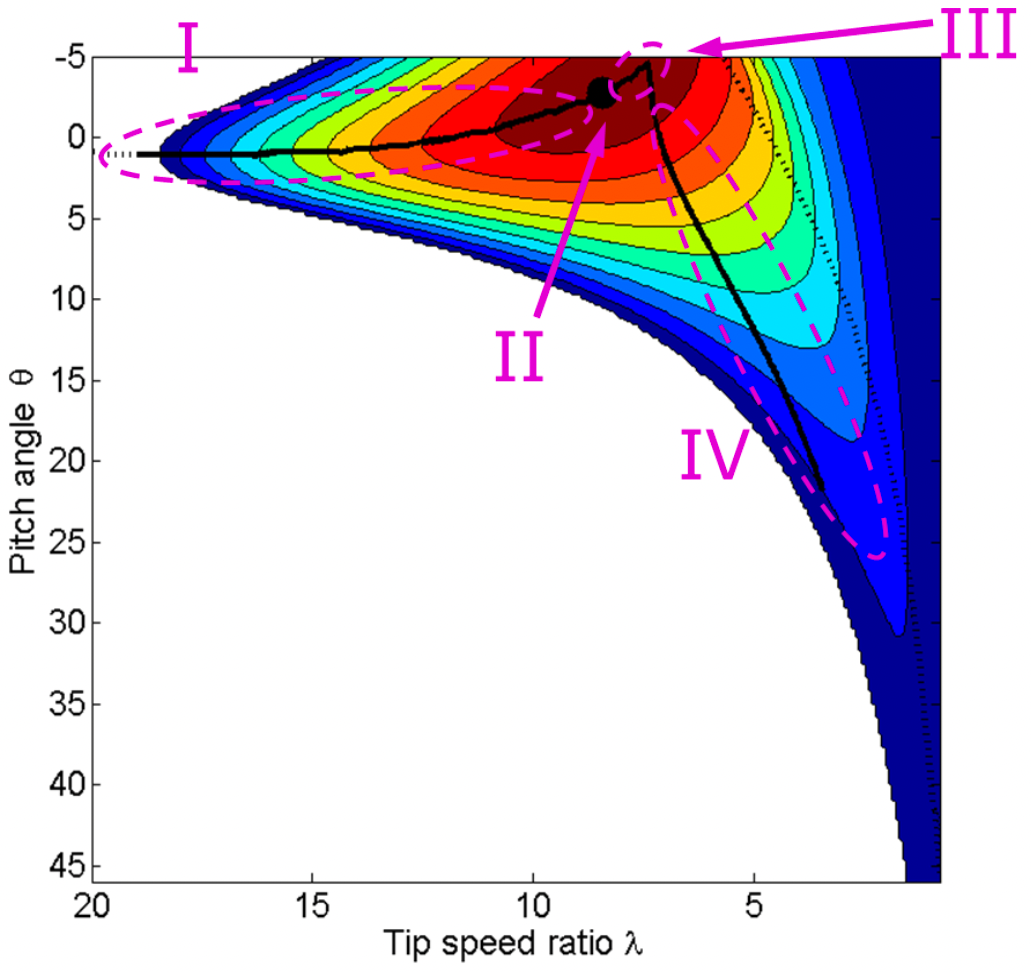
\includegraphics[width=.42\textwidth]{../Graphics/Cp2dPlotRegions.png}%
			\label{fig:cp_plot2d}}
		\label{fig:cp_plot}
	\end{figure}
\end{frame}

%%%%%%%%%%%%%%%%%%

\begin{frame}{Theoretical Background}{Full load control}
	\begin{itemize}
		\item Constant rotor speed $( \omega_{ref} = \bar \omega )$ and power $( P_{ref} = P_{nom} )$
	\end{itemize}
	\begin{equation}\label{eq:pi_flc_ctrl}
		\theta_{ref} = K_{gs,dP/d\theta} \left(K_{flc,P} \, \omega_e + K_{flc,I} \int \omega_e\right)
	\end{equation}
	Gain scheduling term $ K_{gs,dP/d\theta} $ compensates for non-linear pitch authority
	
	\begin{itemize}
		\item Negative damping due to $ T_g = \dfrac{P_g}{\omega} $ and const $ P_g $
	\end{itemize}
	\begin{equation}\label{eq:rotor_speed_deriv_2}
		\dot{\Omega} = \dfrac{1}{J} \left( T_r(\theta, v_0) - T_g(P_g, \omega) \right)
	\end{equation}
\end{frame}

%%%%%%%%%%%%%%%%%%

\begin{frame}{Theoretical Background}{FOWT challenges and control}
	\begin{equation} \label{eq:aero_thrust}
		F_T(\theta, \Omega, v) = \dfrac{1}{2} \rho A_d v^2 C_T(\theta, \Omega, v)
	\end{equation}
	Rotor thrust vs. wind speed with active controller.
	\begin{figure}[ht]
		\centering
		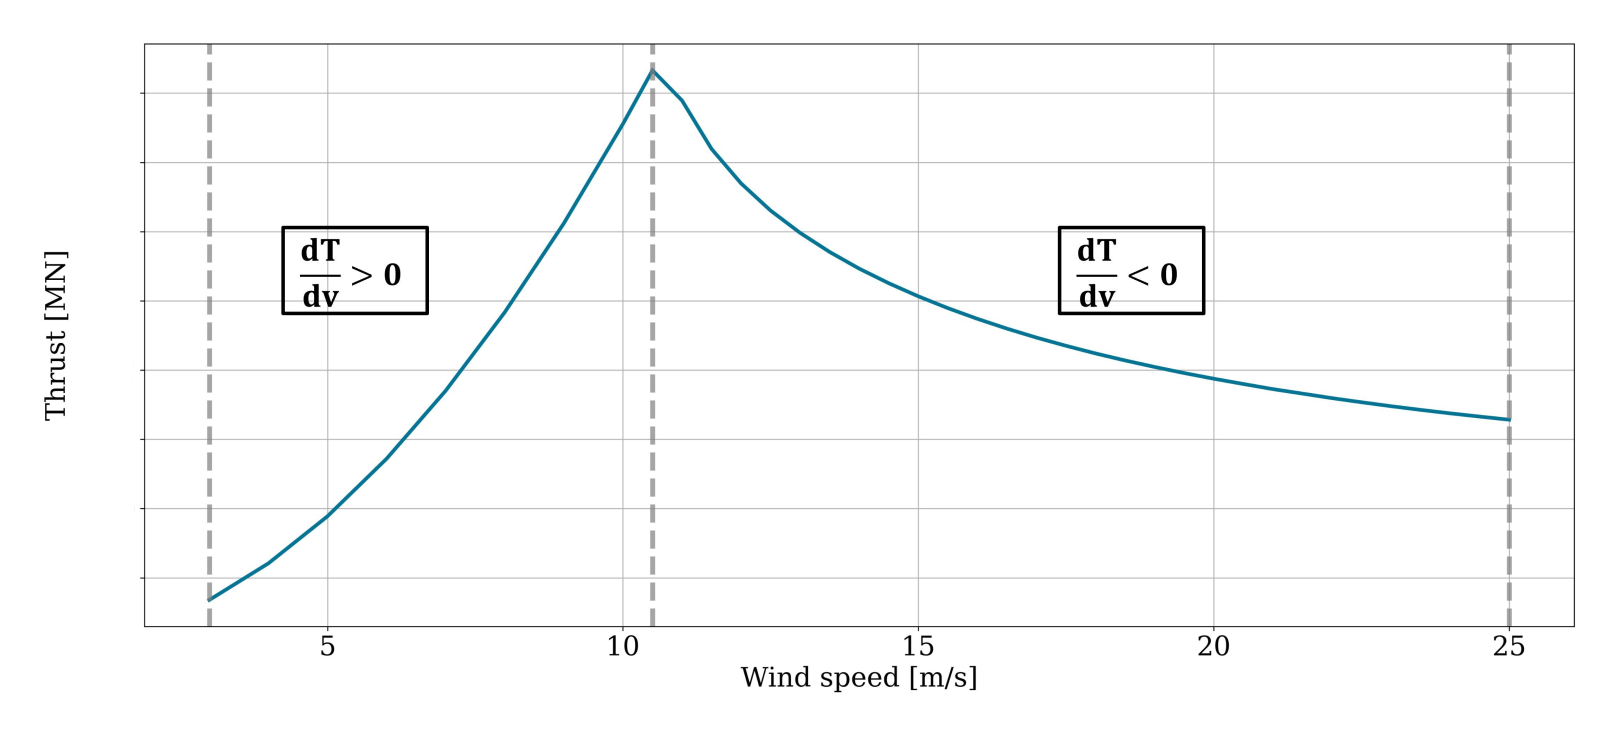
\includegraphics[width=0.85\linewidth]{../Graphics/ThrustWindpeedCurve.PNG}
		\label{fig:thrust_vs_windspeed}
	\end{figure}

	\begin{itemize}
		\item The negative damping problem
	\end{itemize}
	\begin{equation}\label{eq:vrot}
		v_{rot} = v_0 - v_y
	\end{equation}
\end{frame}

%%%%%%%%%%%%%%%%%%

\begin{frame}{Theoretical Background}{Negative damping problem}
	FLC and FATD have contradicting goals
	
	\smallskip
	In most FLC operating range: $ \dfrac{\partial T_r}{\partial \theta} < 0 $ which means $ \dfrac{\partial \Omega}{\partial \theta} < 0 $ but also $ \dfrac{\partial F_T}{\partial \theta} < 0 $ 

	\smallskip
	An example:
	\begin{enumerate}
		\item The turbine is moving forward: $ v_y < 0 $
		\item Thus $ \dfrac{\partial \Omega}{\partial v_{rot}} > 0 $ and consequently $ \Omega > \Omega_{ref} $
		\item FLC: $ \dot \theta_{ref} > 0 \rightarrow \dot \Omega < 0 $ and FATD: $ \dot \theta_{ref} < 0 \rightarrow \dot F_T > 0 $
	\end{enumerate}

\end{frame}

%%%%%%%%%%%%%%%%%%

%%%%%%%%%%%%%%%%%%
%\begin{frame}{Big header}{Smaller header}
%	\textbf{Some text}
%	\begin{itemize}
%		\item Item
%	\end{itemize}
%\end{frame}
%
